\documentclass[runningheads]{llncs}
\usepackage{algorithm,algorithmic,amsfonts,bm,booktabs,tikz,pgf,pgfplots,amsmath,soul,url,graphicx,amsmath,booktabs,booktabs,nicefrac,bm,colortbl,tikz,pgfplots,enumerate,xargs,optidef}
\usetikzlibrary{arrows,automata,circuits}
%\captionsetup{compatibility=false}
\usetikzlibrary{arrows,plotmarks,decorations.markings,trees,shapes}
\tikzstyle{nodo}=[ellipse,draw=black!100,fill=black!30,line width=.7pt,minimum width=1.2cm,minimum height=.7cm]
\tikzstyle{Qnodo}=[ellipse,draw=black!100,fill=black!10,line width=.7pt,minimum width=1.2cm,minimum height=.7cm]
\tikzstyle{arco}=[draw=black!80,line width=.7pt, postaction={decorate}, decoration={markings,mark=at position 1.0 with {\arrow[ draw=black!80,line width=.7pt]{>}}}]
\tikzstyle{decision} = [rectangle, draw, fill=black!100,text=white, text width=4.5em, text badly centered, node distance=3cm, minimum height=3em]
\tikzstyle{block} = [rectangle, draw, fill=blue!20, text width=5em, text centered, rounded corners, minimum height=3em]
\tikzstyle{line} = [draw, -latex']
\tikzstyle{cloud} = [draw, ellipse,fill=red!20, node distance=3cm, minimum height=2em]
\def\mystrut{\vphantom{hg}}
\pgfplotsset{legend image with text/.style={
legend image code/.code={%
\node[anchor=center] at (0.3cm,0cm) {#1};}},}
\pgfplotsset{compat=1.13}
\begin{document}
\title{A New Score for Adaptive Tests\\ in Bayesian and Credal Networks}
\author{Alessandro Antonucci \and
Francesca Mangili \and \\
Claudio Bonesana \and
Giorgia Adorni}
%%\thanks{Supported by organization x.}}
%\titlerunning{A New ScoreAbbreviated paper title}
\authorrunning{Antonucci et al.}
\institute{Istituto Dalle Molle di Studi sull'Intelligenza Artificiale, Lugano, Switzerland
\email{\{alessandro,francesca,claudio.bonesana,giorgia.adorni\}@idsia.ch}}
\maketitle
\begin{abstract}
A test is \emph{adaptive} when its sequence and number of questions is dynamically tuned on the basis of the estimated skills of the taker. Graphical models, such as Bayesian networks, are used for adaptive tests as they allow to model the uncertainty about the questions and the skills in an explainable fashion, especially when coping with multiple skills. A better elicitation of the uncertainty in the question/skills relations can be achieved by interval probabilities. This turns the model into a \emph{credal} network, thus making more challenging the inferential complexity of the queries required to select questions. This is especially the case for the information theoretic quantities used as \emph{scores} to drive the adaptive mechanism. We present an alternative family of scores, based on the mode of the posterior probabilities, and hence easier to explain. This makes considerably simpler the evaluation in the credal case, without significantly affecting the quality of the adaptive process. Numerical tests on synthetic and real-world data are used to support this claim.
\keywords{computer adaptive tests \and information theory \and credal networks \and Bayesian networks \and index of qualitative variation}
\end{abstract}
\section{Introduction}\label{sec:intro}
A test or an exam can be naturally intended as a measurement process, with the questions acting as sensors measuring the skills of the test taker in a particular discipline. Such measurement is typically imperfect with the skills modelled as latent variables whose actual values cannot be revealed in a perfectly reliable way. The role of the questions, whose answers are regarded instead as manifest variables, is to reduce the uncertainty about the latent skills. Following this perspective, probabilistic models are an obvious framework to describe tests. Consider for instance the example in Figure \ref{fig:minicat}, where a Bayesian network evaluates the probability that the test taker knows how to multiply integers. In such framework making the test \emph{adaptive}, i.e., picking a next question on the basis of the current knowledge level of the test taker is also very natural. The information gain for the available questions might be used to select the question leading to the more informative results (e.g., according to Table \ref{tab:minicat}, $Q_1$ is more informative than $Q_2$ no matter what the answer is). This might also be done before the answer on the basis of expectations over the possible alternatives.

A critical point when coping with such approaches is to provide a realistic assessment for the probabilistic parameters associated with the modelling of the relations between the questions and the skills. Having to provide sharp numerical values for these probabilities might be difficult. As the skill is a latent quantity, complete data are not available for a statistical learning and a direct elicitation should be typically demanded to experts (e.g., a teacher). Yet, it might be not obvious to express such a domain knowledge by single numbers and a more robust elicitation, such as a probability interval (e.g., $P(Q_1=1|S_1=1)\in[0.85,0.95]$), might add realism and robustness to the modelling process \cite{hajek2012rationality}. With such generalized assessments of the parameters a Bayesian network simply becomes a \emph{credal} network \cite{antonucci2010d}. The counterpart of such increased realism is the higher computational complexity characterizing inference in credal networks \cite{maua14jair}. This is an issue especially when coping with information theoretic measures such an information gain, whose computation in credal networks might lead to complex non-linear optimization tasks \cite{mangili2017b}. The goal of this paper is to investigate the potential of alternatives to the information-theoretic scores driving the question selection in adaptive tests based on directed graphical models, no matter whether these are Bayesian or credal networks. In particular, we consider a family of scores based on the (expected) mode of the posterior distributions over the skills. We show that, when coping with credal networks, the computation of these scores can be reduced to the simpler optimization tasks involving multi-linear optimizations for which powerful approximation schemes are already available \cite{antonucci2013a}. Moreover, we show that these scores benefit of better explainability properties, thus allowing for a more transparent process in the question selection.

\begin{figure}[htp!]
\centering
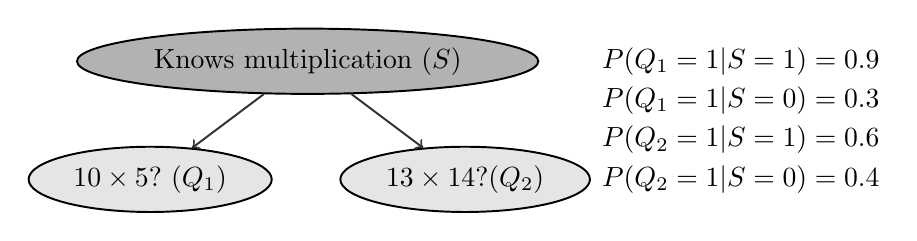
\begin{tikzpicture}[scale=1]
%\node[] ()  at (4,0.5) {\tiny $P(S=1)=0.5$};
\node[] ()  at (5.5,0.5) {$P(Q_1=1|S=1)=0.9$};
\node[] ()  at (5.5,0.) {$P(Q_1=1|S=0)=0.3$};
\node[] ()  at (5.5,-0.5) {$P(Q_2=1|S=1)=0.6$};
\node[] ()  at (5.5,-1.) {$P(Q_2=1|S=0)=0.4$};
\node[nodo] (s)  at (0,0.5) {Knows multiplication ($S$)};
\node[Qnodo] (q1)  at (-2.,-1) {$10\times 5?$ ($Q_1$)};
\node[Qnodo] (q2)  at (+2,-1) {$13\times 14?$($Q_2$)};
\draw[arco] (s) -- (q1);
\draw[arco] (s) -- (q2);
\end{tikzpicture}
\caption{A Bayesian network over Boolean variables modelling a simple test to evaluate integer multiplication skill with two questions.}
\label{fig:minicat}
\end{figure}
\begin{table}[htbp!]
\centering
\caption{Posterior probabilities of the skill after one or two questions in the test based on the Bayesian network in Figure \ref{fig:minicat}. A uniform prior over the skill is considered. Probabilities are regarded as grades and sorted from the lowest one. Bounds to a perturbation $\epsilon=\pm 0.05$ of all the model input parameters are also reported.}
\begin{tabular}{@{}ccrrr@{}}
\toprule
$Q_1$&$Q_2$&$P(S=1|q_1,q_2)$&
$\underline{P}(S=1|q_1,q_2)$&
$\overline{P}(S=1|q_1,q_2)$
\\
\midrule
$0$&$0$&$0.087$&$0.028$&$0.187$\\
$0$&$-$&$0.125$&$0.052$&$0.220$\\
$0$&$1$&$0.176$&$0.092$&$0.256$\\
$-$&$0$&$0.400$&$0.306$&$0.506$\\
$-$&$1$&$0.600$&$0.599$&$0.603$\\
$1$&$0$&$0.667$&$0.626$&$0.708$\\
$1$&$-$&$0.750$&$0.748$&$0.757$\\
$1$&$1$&$0.818$& $0.784$ &$0.852$\\
\bottomrule
\end{tabular}
\label{tab:minicat}
\end{table}
The paper is organized as follows. A critical discussion about the existing work in this area is in Section \ref{sec:work}. The necessary background material is reviewed in Section \ref{sec:background}. The adaptive testing concepts are introduced in Section \ref{sec:cat} and specialized to graphical models in \ref{sec:bncat}. The technical part of the paper is in Section \ref{sec:mode}, where the new scores are discussed and specialized to the credal case, while the experiments are in Section \ref{sec:exp}. Conclusions and outlooks are in Section \ref{sec:conc}.

\section{Related Work}\label{sec:work}
Modelling a test as a process relating latent and manifest variables since the classical \emph{item response theory}, that has been widely used even to implement adaptive sequences \cite{embretson2013item}. Despite its success related to the ease of implementation and inference, IRT might be inadequate when coping with multiple latent skill, especially when these are dependent. This led researchers towards the area of probabilistic graphical models as tools to implement IRT in more complex setups \cite{mislevy1997graphical}. Eventually, Bayesian networks have been identified as a natural framework to models tests, even behind the IRT framework \cite{vomlel2004bayesian}, this being especially the case for adaptive models \cite{vomlel2004building} and coached solving \cite{conati1997line}. In order to cope with latent skills, some authors explored the application of EM-like approaches to these models \cite{plajner2020monotonicity}, this also involving the extreme situation of no ground truth information about the answers \cite{bachrach2012grade}.
As an alternative approach to the same issue, some authors considered relaxations of the Bayesian formalism, such as fuzzy models \cite{badaracco2013fuzzy} and imprecise probabilities \cite{mangili2017b}. This latter direction is the same direction we consider, but trying to overcome the computational limitations of that approach when coping with information-theoretic scores. Compared to the approach in \cite{chen2015computer}, that is focused in the Bayesian case only, we are interested in measures that could easily extended to the imprecise probability framework, this not being the case of the same-decision problem considered in that work.

\section{Background on Bayesian and Credal Networks}\label{sec:background}
We denote variables by Latin uppercase letters, while using lowercase for their generic values, and calligraphic for the set of their possible values. Thus, $x \in \mathcal{X}$ is a possible value of $X$. Here we only consider discrete variables.\footnote{IRT uses instead with continuous skills. Yet, when coping probabilistic models, having discrete skill does no prevent evaluations to range over a continuous domain. E.g., see Table \ref{tab:minicat}, where the grade corresponds to a (continuous) probability.}

\subsection{Bayesian Networks}
A probability mass function (PMF) over $V$ is denoted as $P(V)$, while $P(v)$ is the probability assigned to state $v$. Given a function $f$ of $V$, its expectation with respect to $P(V)$ is $\mathbb{E}_P(f):=\sum_{v\in\mathcal{V}} P(v) \cdot f(v)$. The expectation of $-\log_b[P(V)]$ is called \emph{entropy} and denoted also as $H(X)$.\footnote{We set $0 \cdot \log_b 0 = 0$ to cope with zero probabilities.} We set $b:=|\mathcal{V}|$ to have the maximum of the entropy, achieved for uniform PMFs, equal to one.

Given joint PMF $P(U,V)$, the marginal PMF $P(V)$ is obtained by summing out the other variable, i.e., $P(v)=\sum_{u\in\mathcal{U}} P(u,v)$. Conditional PMFs such as $P(U|v)$ are similarly obtained by Bayes's rule, i.e., $P(u|v)=P(u,v)/P(v)$ provided that $P(v)>0$. Notation $P(U|V):=\{P(U|v)\}_{v\in\mathcal{V}}$ is used for such conditional probability table (CPT). The entropy of a conditional PMF is defined as in the unconditional case and denoted as $H(U|v)$. The conditional entropy is a weighted average of entropies of the conditional PMFs, i.e., $H(U|V):=\sum_{v\in\mathcal{V}} H(U|v) P(v)$. If $P(u,v)=P(u) P(v)$ for each $u\in\mathcal{U}$ and $v\in\mathcal{V}$, variables $U$ and $V$ are independent. Conditional formulations are also considered.

We assume the set of variables $\bm{V}:=(V_1,\ldots,V_r)$ to be in one-to-one correspondence with a directed acyclic graph $\mathcal{G}$. For each $V\in\bm{V}$, the parents of $V$, i.e., the predecessors of $V$ in  $\mathcal{G}$, are denoted as $\mathrm{Pa}_V$. Graph $\mathcal{G}$ together with the collection of CPTs $\{P(V|\mathrm{Pa}_V)\}_{V\in\bm{V}}$ provides a Bayesian network (BN) specification \cite{koller2009}. Under the Markov condition, that states that every variable is conditionally independent of its non-descendants non-parents given its parents, a BN compactly defines a joint PMF $P(\bm{V})$ that factorizes as $P(\bm{v})=\prod_{V\in\bm{V}} P(v|\mathrm{pa}_V)$. Inference intended as the computation of the posterior PMF of a single (queried) variables given some evidence about other variables is in general NP-hard, but exact and approximate schemes are available (see \cite{koller2009} for details).

\subsection{Credal Sets and Credal Networks}
A set of PMFs over $V$ is denoted as $K(V)$ and called \emph{credal set} (CS). Expectations based on CSs are the bounds of the PMF expectations with respect to the CS. Thus $\underline{\mathbb{E}}[f]:=\inf_{P(V)\in K(V)} \mathbb{E}[f]$ and similarly for the supremum $\overline{\mathbb{E}}$. Expectations of events are in particular caller lower and upper probabilities and denoted as $\underline{P}$ and $\overline{P}$. Notation $K(U|v)$ is used for a set of conditional CSs, while $K(U|V):=\{K(U|v)\}_{v\in\mathcal{V}}$ is a credal CPT (CCPT).

Analogously to a BN, a credal network (CN) is specified by graph $\mathcal{G}$ together with a family of CCPTs $\{K(V|\mathrm{Pa}_V)\}_{V\in\bm{V}}$ \cite{cozman2000}. A CN defines a joint CS $K(\bm{V})$ corresponding to all the joint PMFs induced by BNs whose CPTs are consistent with the CN CCPTs. For CNs, we intend inference as the computation of the lower and upper posterior probabilities. The task generalizes BN inference being therefore NP-hard, see  \cite{maua2014jair} for a deeper characterization.

\section{Testing Algorithms}\label{sec:cat}
A typical test aims at evaluating the knowledge level of a test taker $\sigma$ on the basis of her answers to a number of questions. Let $\bm{Q}$ denote a repository of questions available to the instructor. The order and the number of questions picked from $\bm{Q}$ to be asked to $\sigma$ might not be defined in advance. We call \emph{testing algorithm} (TA) a procedure taking care of the selection of the sequence of questions asked to the test taker, and to decide when the test stops. Algorithm \ref{alg:ta} depicts a general TA scheme, with $\bm{e}$ denoting the array of the answers collected from test taker $\sigma$.

\begin{algorithm}[htp!]
\begin{algorithmic}[1]
\STATE $\bm{e}\gets\emptyset$
\WHILE{ {\bf not} $\tt{Stopping}(\bm{e})$}
\STATE $Q^* \gets \tt{Pick}(\bm{Q},\bm{e})$
\STATE $q^* \gets {\tt{Answer}}(Q^*,\sigma)$
\STATE $\bm{e} \gets \bm{e} \cup \{ Q^*=q^* \}$
\STATE $\bm{Q} \gets \bm{Q} \setminus \{ Q^*\}$
\ENDWHILE
\STATE {\bf return} $\tt{Evaluate}(\bm{e})$
\end{algorithmic}
\caption{General TA: given the profile $\sigma$ and repository $\bm{Q}$, an evaluation based on answers $\bm{e}$ is returned.\label{alg:ta}}
\end{algorithm}

Boolean function ${\tt Stopping}$ decides whether the test should end, this choice being possibly based on the previous answers in $\bm{e}$. Trivial stopping rules might be based on the number of questions asked to the test takes (${\tt Stopping}(\bm{e})=1$ if and only if $|\bm{e}|>n$) or on the number of correct answers provided that a maximum number of questions is not exceeded. Function ${\tt Pick}$ selects instead the question to be asked to the student from the repository $\bm{Q}$. A TA is called \emph{adaptive} when this function takes into account the previous answers $\bm{e}$. Trivial non-adaptive strategies might consist in randomly picking an element of $\bm{Q}$ or following a fixed order. Function ${\tt Answer}$ is simply collecting (or simulating) the answer of test taker $\sigma$ to a particular question $Q$. In our assumptions, this answer is not affected by the previous answers to other questions.\footnote{Generalized setups where the quality of the student answer is affected by the previous answers will be discussed at the end of the paper. This might include a \emph{fatigue} model negatively affecting the quality of the answers when many questions have been already answered as well as the presence of \emph{revealing} questions that might improve the quality of other answers \cite{laitusis2007examination}.} 

Finally, ${\tt Evaluate}$ is a function returning the overall judgement of the test (e.g., a numerical grade or a pass/fail Boolean) on the basis of all the answers collected after the test termination. Trivial examples of such functions are the percentage of correct answers or a Boolean that is true when a sufficient number of correct answers has been provided. Note also that in our assumptions the TA is \emph{exchangeable}, i.e., the stopping rule, the question finder and the evaluation function are invariant with respect to permutations in $\bm{e}$ \cite{sawatzky2016accuracy}. In other words, the same next question, the same evaluation and the same stopping decision is produced for any two students, who provided the same list of answers in two different orders.

A typical TA is required to achieve a reliable evaluation of the student $\sigma$ after the answers $\bm{e}$. As each answer is individually assumed to improve such quality, asking all the questions, no matter in which  order because of the exchangeability assumption, is an obvious choice. Yet, this might be impractical (e.g., because of time limitations) or just provide an unnecessary burden to the test taker. The goal of a good TA is therefore to trade off the accuracy of the evaluation and the number of questions.\footnote{In some generalized setups, other elements such as a \emph{serendipity} in choice in order to avoid tedious sequences of questions might be also considered \cite{badran2019adaptive}.}

\section{Adaptive Testing in Bayesian and Credal Networks}\label{sec:bncat}
The general TA setup in Algorithm \ref{alg:ta} can be easily specialized to BNs as follows. First, we identify the profile $\sigma$ of the test taker with the actual states of a number of latent discrete variables, called \emph{skills}. Let $\bm{S}=\{S_i\}_{j=1}^n$ denote these skill variables, and $\bm{s}_\sigma$ the actual values associated with the test take. Skills are typically ordinal variables, whose states corresponds to increasing knowledge levels. Questions in $\bm{Q}$ are still described as manifest variables whose actual values are returned by the {\tt answer} function. This is achieved by a (possibly stochastic) function of the actual profile $\bm{s}_\sigma$. Thus reflect the taker perspective, while the teacher has clearly no access to $\bm{s}_\sigma$. As a remark, note that we might coarsen the set of possible values $\mathcal{Q}$ each $Q\in \bm{Q}$: for instance, a multiple choice question with three options might have a single right, the two other answers being indistinguishable from the evaluation point of view.\footnote{The case of \emph{abstention} to an answer and the consequent problem of modelling the incompleteness is a topic we do not consider here for the sake of conciseness. Yet, general approaches in the spirit of xxx could be naturally considered.} 
 
A joint PMF over the skills $\bm{S}$ and the questions $\bm{Q}$ is supposed to be available. In particular we assume this to correspond to a BN whose graph has the questions as leaf nodes. Thus, for each $Q\in\bm{Q}$, $Pa_Q \subseteq \bm{S}$ and we call $Pa_Q$ the \emph{scope} of question $Q$. Note that this assumption about the graph is simply reflecting a statement about the conditional independence between (the answer to) a question and all the other skills and questions given scope of the question. This basically means that the answers to other questions are not directly affecting the answer to a particular question, and this naturally follows from the exchangeability assumption.\footnote{Moving to other setups would not really be critical because of the property of observed nodes in Bayesian and credal networks, see for instance \cite{antonucci2009,bolt}.}

As the available data are typically incomplete because of the latent nature of the skills, dedicated learning strategies, such as various form of constrained EM should be considered to train a BN from data. We refer the reader to the various contributions of Plajner and Vomlel in this field (e.g., \cite{plajner2020monotonicity}) for a complete discussion of that approach. Here we assume the BN quantification already available.

In such a BN framework, ${\tt Stopping}(\bm{e})$ might be naturally based on an evaluation of the posterior PMF $P(\bm{S}|\bm{Q}=\bm{e})$, this being also the case for ${\tt Evaluate}$. Regarding the question selection, ${\tt Pick}$ might be similarly based on the (posterior) CPT $P(\bm{S}|Q,\bm{Q}=\bm{e})$, whose values for the different answers to $Q$ might be weighted by the marginal $P(Q|\bm{e})$. More specifically, entropies and conditional entropies are considered by Algorithm \ref{alg:bnta}, while the evaluation is based on a conditional expectation for a given utility function.

\begin{algorithm}[htp!]
\begin{algorithmic}[1]
\STATE $\bm{e}=\emptyset$
\WHILE{ {\bf not} $H(\bm{X}|\bm{e}) > H^*$}
\STATE $Q^* \gets \arg\max_{Q \in \bm{Q}} H(\bm{S}|Q,\bm{Q}=\bm{e})$
\STATE $q^* \gets {\tt{Answer}}(Q^*,\bm{s}_\sigma)$
\STATE $\bm{e} \gets \bm{e} \cup \{ Q^*=q^* \}$
\STATE $\bm{Q} \gets \bm{Q} \setminus \{ Q^*\}$
\ENDWHILE
\STATE {\bf return} $\mathbb{E}_{P(\bm{S}|\bm{e})}[f(\bm{S})]$
\end{algorithmic}
\caption{Information Theoretic TA in BN over the questions $\bm{Q}$ and the skills $\bm{S}$: given the student profile $\bm{s}_\sigma$, the algorithms returns an evaluation corresponding to the expectation of an evaluation function $f$ with respect to the posterior for the skills given the answers $\bm{e}$.\label{alg:bnta}}
\end{algorithm}

When no data can be used for the training, elicitation techniques should be considered instead. As already discussed CNs might offer a better formalism to capture domain knowledge, especially by providing interval-valued probabilities instead of sharp values.
If this is the case, a CN version of Algorithm \ref{alg:bnta} can be equivalently considered. Moving to CN is almost the same, provided that bounds on the entropies are considered instead. Yet, the price of such increased realism in the elicitation is the higher complexity characterizing inferences based on CNs. The work in \cite{mangili2017b} offers a critical discussion of those issues, that are only partially addressed by heuristic techniques used to approximate such bounds. In the next section we conside an alternative approach to cope with CNs and adaptive TAs based on different scores used to select the questions.

\section{Coping with the Mode}\label{sec:mode}
Following \cite{wilcox1973indices} we can regard the PMF entropy (and its conditional version) used by Algorithm \ref{alg:bnta} as an example of index of \emph{qualitative variation} (IQV). An IQV is just a normalized number that takes value zero for degenerate PMFs, one on uniform ones, being independent on the number of possible states (and samples in case of empirical models). The closer to uniform is the PMF, the higher is the index and vice versa.

In order to bypass the computational issues related to its application with CNs and the explainability limits in the general case, here we consder alternative IQVs to replace entropy in Algorithm \ref{alg:bnta}. Wilkox's \emph{deviation from the mode} (DM) appears as a natural choice. For a given PMF $P(X)$, this corresponds to:
\begin{equation}
M(X):=1-\sum_{x\in\mathcal{X}} \frac{\max_{x'\in\mathcal{X}} P(x') - P(x)}{|\mathcal{X}|-1}\,.
\end{equation}
It is a trivial exercise to check that this is a proper IQV, with the same unimodal behaviour of the entropy. Concerning explainability, being a linear function of the modal probability, the numerical value of the DM offers a more transparent interpretation than the entropy. From a computational point of view, for both marginal and unconditional PMFs, both the entropy and DM can be directly obtained from the probabilities of the singletons. 

The situation is different when computing the bounds of these quantities with respect to a CS. The bounds of $M(X)$ are obtained from the upper and lower probabilities of the singletons by simple algebra, i.e,
\begin{equation}
\overline{M}(X):=
\max_{P(X)\in K(X)} M(X):=\frac{|\mathcal{X}|-\max_{x'\in\mathcal{X}} \overline{P}(x')}{|\mathcal{X}|-1}\,.
\end{equation}
and analogously with the upper probabilities for $\overline{M}(X)$. Maximizing entropy requires instead a non-trivial, but convex, optimization. See for instance \cite{abellan2003maximum} for an iterative procedure to find such maximum when coping with CSs defined by probability intervals. The situation is even more critical for the minimization, that has been proved to be NP-hard in \cite{xiang2006estimating}.

The optimization becomes even more challenging for conditional entropies there are roughly mixtures with imprecise weights. Accordingly, in \cite{mangili2017b}, only inner approximation for the upper bound have been derived. The situation is different for conditional DMs. Let us discuss this case in a simplified setup that will be later extended.

\begin{theorem}\label{th:dm}
Under the setup of Section \ref{sec:bncat}, consider a CN with a single skill $S$ and a single question $Q$, that is a child of $S$. Let $K(S)$ and $K(Q|S)$ be the CCPTs of such CN. Let also $\mathcal{Q}=\{q^1,\ldots,q^n\}$ and $\mathcal{S}=\{s^1,\ldots,s^n\}$.
The upper conditional DM, i.e.,
\begin{equation}\label{eq:upperM}
\overline{M}(S|Q):=\max_{\substack{P(S)\in K(S)\\P(Q|S)\in K(Q|S)}} \sum_{i=1,\ldots,n} \left[ \max_{j=1,\ldots,m} P(s_j|q_i) \right] P(q_i)\,,
\end{equation}
is such that:
\begin{equation}\label{eq:upperM2}
\overline{M}(S|Q):=\max_{\substack{\hat{j}_i=1,\ldots,m\\i=1,\ldots,n}} \Omega(\hat{j}_1,\ldots,\hat{j}_n)
%\overline{M}(S|Q):=\max_{\substack{i=1,\ldots,n\\j=1,\ldots,m}} \omega_{ij}
\end{equation}
where $\Omega(\hat{j}_1,\ldots,\hat{j}_n)$ is the solution of the following linear programming task:

\begin{alignat}{3}
\max && \sum_j x_{ij}&&&\nonumber\\
\text{s.t.}\qquad&&\sum_{ij} x_{ij}&=1&& \label{c1}\\
&&x_{ij}&\geq 0&&\qquad \forall i,j \label{c2}\\
&&\sum_{i} x_{ij}&\geq \underline{P}(s_j)&&\qquad \forall j \label{c4}\\
&&\sum_{i} x_{ij}&\leq \underline{P}(s_j)&&\qquad \forall j \label{c5}\\
&&\underline{P}(q_i|s_j) \sum_{i} x_{ij}&\leq x_{ij}&&\qquad \forall i,j \label{c6}\\
&&\overline{P}(q_i|s_j) \sum_{i} x_{ij}&\geq x_{ij}&&\qquad \forall i,j
\label{c7}\\
&&x_{i\hat{j}_i}&\geq x_{ij}&&\qquad \forall i,j \label{c3}
\end{alignat}
where the bounds on the sums over the indexes and on the universal quantifiers.
are omitted for the sake of brevity, 
\begin{proof}
Equation \eqref{eq:upperM} rewrites as:
\begin{equation}\label{eq:firstopt}
\overline{M}(S|Q)
=\max_{\substack{P(S)\in K(S)\\P(Q|S)\in K(Q|S)}} \sum_{i=1}^n \left[ \max_{j=1,\ldots,m} P(s_j)P(q_i|s_j) \right]\,.
\end{equation}
Let us define the variables of such constrained optimization task as:
\begin{equation}
x_{ij}:=P(s_j)P(q_i|s_j)\,.
\end{equation}
for each $i=1,\ldots,n$ and $j=1,\ldots,m$. Let us show how the CCPT constraints can be easily reformulated with respect to such new variables by simply noticing that $x_{ij}=P(s_j,q_i)$, and hence $P(s_i)=\sum_i x_{ij}$ and $P(q_j|s_i)=x_{ij}/(\sum_{k} x_{kj})$. Consequently, the interval constraints on $P(S)$ corresponds to the linear constraints in Equations \eqref{c4} and \eqref{c5}. Similarly, for $P(Q|S)$, we obtain:
\begin{equation}\label{eq:fract}
\underline{P}(q_i|s_j) \leq \frac{x_{ij}}{\sum_k x_{kj}} \leq \overline{P}(q_i|s_j)\,,
\end{equation}
that easily gives the linear constraints in Equations \eqref{c6} and \eqref{c7}.
Finally the non-negativity of the probabilities corresponds to Equation \eqref{c2}, while Equation \eqref{c1} gives the normalization of $P(S)$, while the normalization of $P(Q|S)$ is automatically satisfied. 

Equation \eqref{eq:firstopt} rewrites therefore as:
\begin{equation}\label{eq:lastopt}
\overline{M}(S|Q)
=\max_{ \{v_{ij}\}_{ij} \in \Gamma} \sum_{i} \max_{j} x_{ij} \,,
\end{equation}
where $\Gamma$ denotes the linear constraints in Equations \eqref{c1}-\eqref{c7}. If we set:
\begin{equation}
\hat{j}_i:= \arg \max x_{ij}\,,
\end{equation}
Equation \eqref{eq:lastopt} rewrites as:
\begin{equation}\label{eq:lastopt2}
\overline{M}(S|Q)
=\max_{ \{v_{ij}\}_{ij} \in \Gamma'} \sum_{i} x_{i\hat{j}_i} \,,
\end{equation}
where $\Gamma'$ are the constraints in $\Gamma$ with the additional (linear) constraints in Equation \eqref{c3}.

Yet, the optimization in the right-hand side of Equation \eqref{eq:lastopt2} is not a linear pragramming task, as the values of the indexes $\hat{j}_i$ cannot be decided in advance being potentially different for different assigments of the optimization variables consistent with the constraints in $\Gamma$. Yet, we might address such optimization as a brute-force task with respect to all the possible assignation of the optimal indexes $\hat{j}_i$. This is exactly what is done by Equation \eqref{eq:upperM2} where all the $m^n$ possible assignations are considered. This proves the thesis. \qed
\end{proof}
\end{theorem}

An analogous result with the linear programming tasks minimizing the same objective functions with exactly the same constraints allows to compute $\underline{M}(S|Q)$. 
The overall complexity is clearly $O(m^n)$ with $n:=|\mathcal{Q}|$. This means linear complexity for any test where only the difference between a wrong and a right answer is considered from an elicitation perspective. Extending the result to the case of multiple answers is trivial by means of the results in \cite{antonucci2009}, that allows to merge multiple observed children of a single node into a single one.
Finally, the case of multiple skills might be similarly considered by using the marginal bounds of probabilities for the single skills in Equations \eqref{c4} and \eqref{c5}. 


\section{Experiments}\label{sec:exp}
In this section we validate the ideas outlined in the previous section in order to check whether or not the DM can be used as a sensible alternative to information-theoretic scores such as the entropy in practical TAs. In the BN context, this is simply achieved by computing the necessary updated probabilities, while Theorem \ref{th:dm} is used instead for CNs.

\subsection{Single-Skill Experiments on Synthetic Data}
For a very first validation of our approach, we consider a simple setup made of a single skill $S$ and a repository with 18 Boolean questions based on nine different parametrizations (two questions for parametrization). In the BN, the CPT of a question can be parametrized by two numbers. E.g., in the example in Figure \ref{fig:minicat}, we used the probabilities of correctly answering the question given that the skill is present or not, i.e., $P(Q=1|S=1)$ and $P(Q=1|S=0)$. A more interpretable parametrization can be obtained as follows:
\begin{eqnarray}
\delta &:=& 1-\frac{1}{2}[P(Q=1|S=1)+P(Q=1|S=0)]\,,\\
\kappa &:=& P(Q=1|S=1)-P(Q=1|S=0)\,.
\end{eqnarray}
Note that $P(Q=1|S=1)>P(Q=1|S=0)$ is an obvious rationality constraint for questions, otherwise having the skill would make less likely to answer properly to a question. Both parameters are therefore non-negative. Parameter $\delta$, corresponding to the (arithmetic) average of the probability for a wrong answer over the different skill values, can be regarded as a normalized index of the question \emph{difficulty}. E.g., in Figure \ref{fig:minicat}, $Q_1$ ($\delta=0.4$) is less difficult than $Q_2$ ($\delta=0.5$). Parameter $\kappa$ can be instead regarded as a descriptor of the difference of the conditional PMFs associated with the different skill values. In the most extreme case $\kappa=1$, the CPT $P(Q|S)$ is diagonal implementing an identity mapping between the skill and the question. We therefore regard $\kappa$ as a indicator of the discriminative power of the question. In our tests, for the BN quantifications, we consider the nine possible parametrizations corresponding to $(\delta,\gamma) \in [0.4,0.5,0.6]^2$. For $P(S)$ we use instead a uniform quantification. For the CN approach we perturb all the BN parameters with $\epsilon=\pm 0.05$, thus obtaining a CN quantification. A group of 1024 simulated students, half of them having $S=0$ and half with $S=1$ is used for simulations. The student answers are sampled from the CPT of the asked question on the basis of the student profile. Figure X depicts the accuracy of the BN and CN approaches based on both the entropy and the DM scores, while the Brier score is instead depicted on the left. As baseline, we use the results obtained by randomly picking the questions. As expexted the adaptive aproaches outperform the non-adaptive random approach and, notably, the differences between the two scores seems to be minimal. A closer view can be achieve by considering the Brier score, with the xxx.

%$\lambda:=1-\frac{1}{2}(p_0+p_1)$ and $\delta=(p_1-p_0)$. The first quantity is the arithmetic average of giving a wrong answer and we might indent it as the \emph{level} of the question, this mining that the higher is $\lambda$ the more unlikely is to receive a correct answer is the students have the same probability of having and not having the skill. Regarding $\delta$ we might intend it as the (average) discriminative power of a question.
%Note that the inverse relations give $p_1=1-\lambda+\frac{\delta}{2}$
%and $p_0=1-\lambda-\frac{\delta}{2}$. Where constraint $p_1>p_0$ is just $\delta>0$ and any other value in $[0,1]$ for both parameters is valid.


%The values in the two parameters are xxx in Table X. In the Bayesian case we set $P(S=1)=.5$. The credal model is obtained by a simple contamination with xxx. Two questions for each one of the nine templates are xxx. As stopping rule a threshold on the entropy is set.
%This result allows to apply DM to adaptive TA with both BNs
%*** distinguishing between templates and questions ***

%This makes especially critical the evaluation of the bounds of the entropy. As entropy is a convec function, upper entropy might be found, while the minimization has been proved to be NP-hard by Klir and fast techniques are only available for specific families of CSs. The optimization becomes even more challenging for expected entropies there are roughly mixtures with imprecise weights. Accordingly, in \cite{mangili2017b}, only special cases based on an inner approximation have been derived.
%for each $i,j$. Note that in this case normalization is automatically satisfied and this linear fractional constraint can be 
%\begin{equation}\label{eq:boundsPS}
%\underline{P}(s_j) \leq \sum_i x_{ij} \leq \overline{P}(s_j)\,, 
%\end{equation}
%for each $j$. Normalization of $P(S)$ is therefore:
%\begin{equation}\label{eq:normal}
%\sum_{ij} x_{ij} = 1\,.
%\end{equation}
%Regarding the constraints on $P(Q|S)$: for each $i,j$. Note that in this case normalization is automatically satisfied and this linear fractional constraint can be easily translated into a linear one. Finally, the non-negativity of $P(q_i)$ and $P(s_j|q_i)$ corresponds to the non-negativity of $v_{ij}$. 
%:boundsPS} and \eqref{eq:normal} together with the linearized version of Equation \eqref{eq:fract} and the non-negativity.

%As a first, demonstrative, example of our ideas consider a model characterized by a single (Boolean) Skill $S$ and a set of questions $\bm{Q}$ picked from a set of templates. Let us first focus on a Bayesian, i.e., precise, case. The prior specification $P(S)$ is achieve by a single parameter $p \in [0,1]$ such that $P(S=1)=p$. For a generic question $Q$, which is also assumed to be Boolean, a complete specification of the CPT $P(Q|S)$ is obtained by the two parameters $p_0,p_1\in [0,1]$ where $P(Q=1|S=0)=p_0$ and $P(Q=1|S=1)=p_1$. 
%Consider a PMF $P(X)$. Let $x^*:=\arg\max_{x\in\mathcal{X}} P(x)$. Let %$\mathcal{P}$
%denote the set of all PMFs with the same $p^*:=P(x^*)$. The most entropic %PMF in 
%$\mathcal{P}$ is the one with  $P(x)=\frac{1-p^*}{m-1}$ for each $x\neq %x^*$ where 
%$m:=|\mathcal{X}|$. While the least entropic is the one with a 
%$x'\in\mathcal{X}\setminus\{x^*\}$ such that $P(x')=1-p^*$ and all the %other masses 
%equal to zero. These two bounds on the entropy are therefore:
%\begin{eqnarray}
%\overline{h}&:=& -p^* \log_m p^* - (1-p^*) \log_m \frac{1-p^*}{m-1}\,,\\
%\overline{h}&:=& -p^* \log_m p^* - (1-p^*) \log_m (1-p^*)\,.
%\end{eqnarray}
%This:
%\begin{equation}
%\overline{h}-\underline{h}=(1-p^*) \log_m (m-1)\,,
%\end{equation}
%The maximum gap between the entropies of the PMFs in $\mathcal{P}$ decreases as 
%soon as $p^*$ increases and as soon as the number of states of $X$ decreases, being 
%zero for binary variables.

\begin{figure}[htp!]
\centering
% This file was created by tikzplotlib v0.9.8.
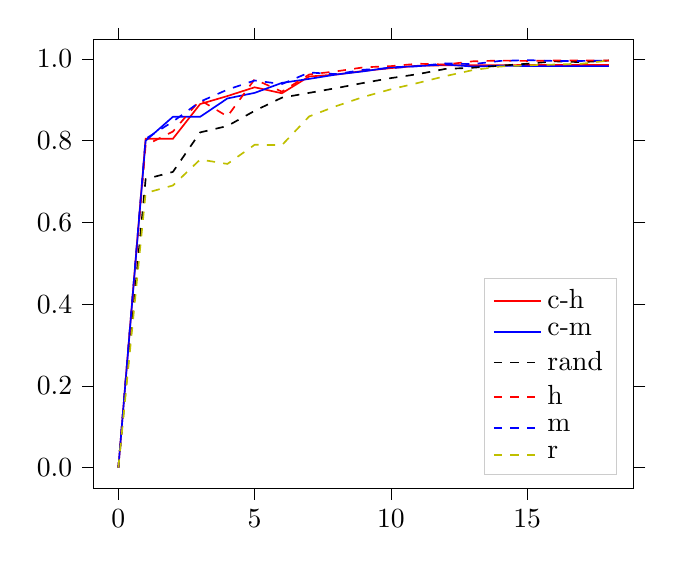
\begin{tikzpicture}

\definecolor{color0}{rgb}{0.75,0.75,0}

\begin{axis}[
legend cell align={left},
legend style={
  fill opacity=0.8,
  draw opacity=1,
  text opacity=1,
  at={(0.97,0.03)},
  anchor=south east,
  draw=white!80!black
},
tick align=outside,
tick pos=both,
x grid style={white!69.0196078431373!black},
xmin=-0.9, xmax=18.9,
xtick style={color=black},
y grid style={white!69.0196078431373!black},
ymin=-0.049853515625, ymax=1.046923828125,
ytick style={color=black},
ytick={-0.2,0,0.2,0.4,0.6,0.8,1,1.2},
yticklabels={−0.2,0.0,0.2,0.4,0.6,0.8,1.0,1.2}
]
\addplot [semithick, red]
table {%
0 0
1 0.8046875
2 0.8046875
3 0.8896484375
4 0.9091796875
5 0.9306640625
6 0.916015625
7 0.95703125
8 0.9619140625
9 0.970703125
10 0.9775390625
11 0.9833984375
12 0.984375
13 0.984375
14 0.984375
15 0.9853515625
16 0.9853515625
17 0.9853515625
18 0.9853515625
};
\addlegendentry{c-h}
\addplot [semithick, blue]
table {%
0 0
1 0.7998046875
2 0.8583984375
3 0.8583984375
4 0.9033203125
5 0.9169921875
6 0.94140625
7 0.951171875
8 0.9619140625
9 0.9697265625
10 0.9794921875
11 0.982421875
12 0.986328125
13 0.9814453125
14 0.9833984375
15 0.982421875
16 0.982421875
17 0.982421875
18 0.982421875
};
\addlegendentry{c-m}
\addplot [semithick, black, dashed]
table {%
0 0
1 0.7060546875
2 0.7236328125
3 0.8203125
4 0.8359375
5 0.873046875
6 0.9052734375
7 0.9169921875
8 0.9287109375
9 0.94140625
10 0.953125
11 0.962890625
12 0.9755859375
13 0.978515625
14 0.9833984375
15 0.98828125
16 0.994140625
17 0.9921875
18 0.99609375
};
\addlegendentry{rand}
\addplot [semithick, red, dashed]
table {%
0 0
1 0.7890625
2 0.822265625
3 0.8994140625
4 0.859375
5 0.9501953125
6 0.919921875
7 0.9619140625
8 0.9697265625
9 0.9794921875
10 0.982421875
11 0.98828125
12 0.986328125
13 0.994140625
14 0.99609375
15 0.9951171875
16 0.99609375
17 0.99609375
18 0.99609375
};
\addlegendentry{h}
\addplot [semithick, blue, dashed]
table {%
0 0
1 0.8046875
2 0.8466796875
3 0.8955078125
4 0.9248046875
5 0.947265625
6 0.9384765625
7 0.966796875
8 0.962890625
9 0.9736328125
10 0.9775390625
11 0.982421875
12 0.9892578125
13 0.9873046875
14 0.9951171875
15 0.9970703125
16 0.9951171875
17 0.9951171875
18 0.99609375
};
\addlegendentry{m}
\addplot [semithick, color0, dashed]
table {%
0 0
1 0.671875
2 0.6904296875
3 0.75390625
4 0.7431640625
5 0.7900390625
6 0.7890625
7 0.859375
8 0.884765625
9 0.9072265625
10 0.92578125
11 0.94140625
12 0.9580078125
13 0.97265625
14 0.9814453125
15 0.984375
16 0.986328125
17 0.98828125
18 0.99609375
};
\addlegendentry{r}
\end{axis}

\end{tikzpicture}

% This file was created by tikzplotlib v0.9.8.
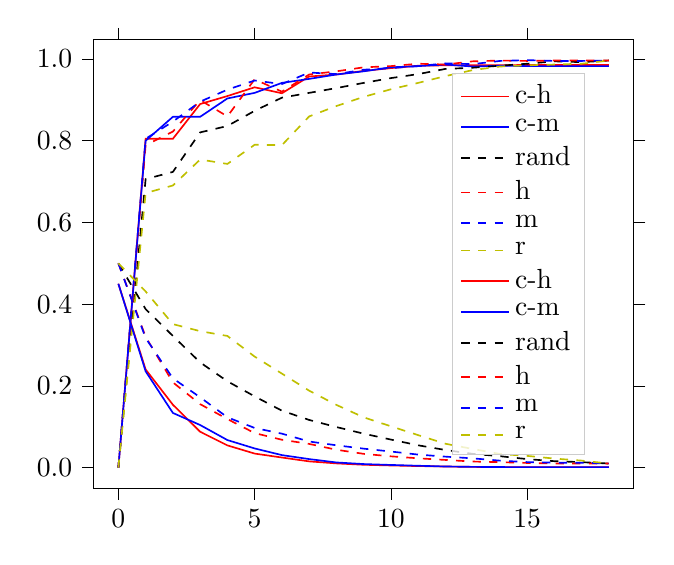
\begin{tikzpicture}

\definecolor{color0}{rgb}{0.75,0.75,0}

\begin{axis}[
legend cell align={left},
legend style={
  fill opacity=0.8,
  draw opacity=1,
  text opacity=1,
  at={(0.91,0.5)},
  anchor=east,
  draw=white!80!black
},
tick align=outside,
tick pos=both,
x grid style={white!69.0196078431373!black},
xmin=-0.9, xmax=18.9,
xtick style={color=black},
y grid style={white!69.0196078431373!black},
ymin=-0.049853515625, ymax=1.046923828125,
ytick style={color=black},
ytick={-0.2,0,0.2,0.4,0.6,0.8,1,1.2},
yticklabels={−0.2,0.0,0.2,0.4,0.6,0.8,1.0,1.2}
]
\addplot [semithick, red]
table {%
0 0
1 0.8046875
2 0.8046875
3 0.8896484375
4 0.9091796875
5 0.9306640625
6 0.916015625
7 0.95703125
8 0.9619140625
9 0.970703125
10 0.9775390625
11 0.9833984375
12 0.984375
13 0.984375
14 0.984375
15 0.9853515625
16 0.9853515625
17 0.9853515625
18 0.9853515625
};
\addlegendentry{c-h}
\addplot [semithick, blue]
table {%
0 0
1 0.7998046875
2 0.8583984375
3 0.8583984375
4 0.9033203125
5 0.9169921875
6 0.94140625
7 0.951171875
8 0.9619140625
9 0.9697265625
10 0.9794921875
11 0.982421875
12 0.986328125
13 0.9814453125
14 0.9833984375
15 0.982421875
16 0.982421875
17 0.982421875
18 0.982421875
};
\addlegendentry{c-m}
\addplot [semithick, black, dashed]
table {%
0 0
1 0.7060546875
2 0.7236328125
3 0.8203125
4 0.8359375
5 0.873046875
6 0.9052734375
7 0.9169921875
8 0.9287109375
9 0.94140625
10 0.953125
11 0.962890625
12 0.9755859375
13 0.978515625
14 0.9833984375
15 0.98828125
16 0.994140625
17 0.9921875
18 0.99609375
};
\addlegendentry{rand}
\addplot [semithick, red, dashed]
table {%
0 0
1 0.7890625
2 0.822265625
3 0.8994140625
4 0.859375
5 0.9501953125
6 0.919921875
7 0.9619140625
8 0.9697265625
9 0.9794921875
10 0.982421875
11 0.98828125
12 0.986328125
13 0.994140625
14 0.99609375
15 0.9951171875
16 0.99609375
17 0.99609375
18 0.99609375
};
\addlegendentry{h}
\addplot [semithick, blue, dashed]
table {%
0 0
1 0.8046875
2 0.8466796875
3 0.8955078125
4 0.9248046875
5 0.947265625
6 0.9384765625
7 0.966796875
8 0.962890625
9 0.9736328125
10 0.9775390625
11 0.982421875
12 0.9892578125
13 0.9873046875
14 0.9951171875
15 0.9970703125
16 0.9951171875
17 0.9951171875
18 0.99609375
};
\addlegendentry{m}
\addplot [semithick, color0, dashed]
table {%
0 0
1 0.671875
2 0.6904296875
3 0.75390625
4 0.7431640625
5 0.7900390625
6 0.7890625
7 0.859375
8 0.884765625
9 0.9072265625
10 0.92578125
11 0.94140625
12 0.9580078125
13 0.97265625
14 0.9814453125
15 0.984375
16 0.986328125
17 0.98828125
18 0.99609375
};
\addlegendentry{r}
\addplot [semithick, red]
table {%
0 0.449999999999992
1 0.240321093750003
2 0.154068750000002
3 0.0879601562499998
4 0.0545979492187504
5 0.0345669921874999
6 0.0248742187499998
7 0.0154591796875
8 0.0104958984375
9 0.00716503906250006
10 0.00544667968750006
11 0.00400634765625
12 0.00290869140625
13 0.00200585937499999
14 0.00137460937499999
15 0.00145478515624999
16 0.00144414062499999
17 0.00143984374999999
18 0.00143974609374999
};
\addlegendentry{c-h}
\addplot [semithick, blue]
table {%
0 0.449999999999992
1 0.235816308593751
2 0.133981542968751
3 0.1044369140625
4 0.0676275390624998
5 0.0471173828125
6 0.0308186523437499
7 0.0210914062499999
8 0.0128307617187499
9 0.00890488281249997
10 0.00674853515625
11 0.00476650390625
12 0.00295224609375002
13 0.00205888671875
14 0.00155673828125
15 0.00136240234375
16 0.00144453125
17 0.0014396484375
18 0.001439453125
};
\addlegendentry{c-m}
\addplot [semithick, black, dashed]
table {%
0 0.5
1 0.38800205078125
2 0.32236396484375
3 0.25762578125
4 0.21144267578125
5 0.1745076171875
6 0.139484375
7 0.116849609375
8 0.09946396484375
9 0.0832636718750001
10 0.0688158203125002
11 0.0547997070312502
12 0.0433041015625001
13 0.0339080078125
14 0.0281607421874999
15 0.0210115234374999
16 0.0159416015625
17 0.013575390625
18 0.0101943359375
};
\addlegendentry{rand}
\addplot [semithick, red, dashed]
table {%
0 0.5
1 0.3201904296875
2 0.20880224609375
3 0.155491015625001
4 0.118972656250001
5 0.0846564453125002
6 0.0683878906250001
7 0.0581800781250001
8 0.04395986328125
9 0.0338941406249999
10 0.0278213867187499
11 0.0230004882812499
12 0.01899560546875
13 0.0150919921875
14 0.0135923828125
15 0.0116212890625
16 0.01030810546875
17 0.0101529296875
18 0.0101943359375
};
\addlegendentry{h}
\addplot [semithick, blue, dashed]
table {%
0 0.5
1 0.317187499999997
2 0.218678808593748
3 0.172235253906248
4 0.123334277343749
5 0.0972216796875
6 0.0832712890624999
7 0.0641038085937499
8 0.0548044921874999
9 0.04663076171875
10 0.03955947265625
11 0.0320949218749999
12 0.0270456054687499
13 0.0228884765625
14 0.0172658203125
15 0.01367705078125
16 0.0123193359375
17 0.01206787109375
18 0.0101943359375
};
\addlegendentry{m}
\addplot [semithick, color0, dashed]
table {%
0 0.5
1 0.431250000000002
2 0.351269531249998
3 0.3340296875
4 0.322312109375
5 0.27181015625
6 0.23018603515625
7 0.188451464843749
8 0.15362529296875
9 0.123285546875
10 0.10120791015625
11 0.0796852539062503
12 0.0586057617187502
13 0.0458888671875001
14 0.0336228515625
15 0.02890341796875
16 0.022294140625
17 0.01733564453125
18 0.0101943359375
};
\addlegendentry{r}
\end{axis}

\end{tikzpicture}

\caption{Aggregated Accuracy (left) and Brier score (right) for a single-skill TA}
\label{fig:mono}
\end{figure}
\subsection{Multi-Skill Experiments on Real Data}
For a validation on real data, we consider data about online German language placement (see also \cite{mangili2017b}). Four different Boolean skills associated with different abilities (vocabulary, communication, listening and reading) are considered and modeled by a chain-shaped graph, for which BN and CN quantification are already available. Experiments have been achieved by means of the CREMA library for credal networks \cite{huber2020a}.\footnote{github.com/IDSIA/crema} The Java code used for the modelling and the simulations is available together with the Python scripts used to analyze the results.\footnote{github.com/IDSIA/adaptive-tests}. Results are depicted with the same spirit of those in Section X in Figure xxx. Notably, even with multiple skills, we obtain similar results xxx. 

\begin{figure}[htp!]
\centering
% This file was created by tikzplotlib v0.9.8.
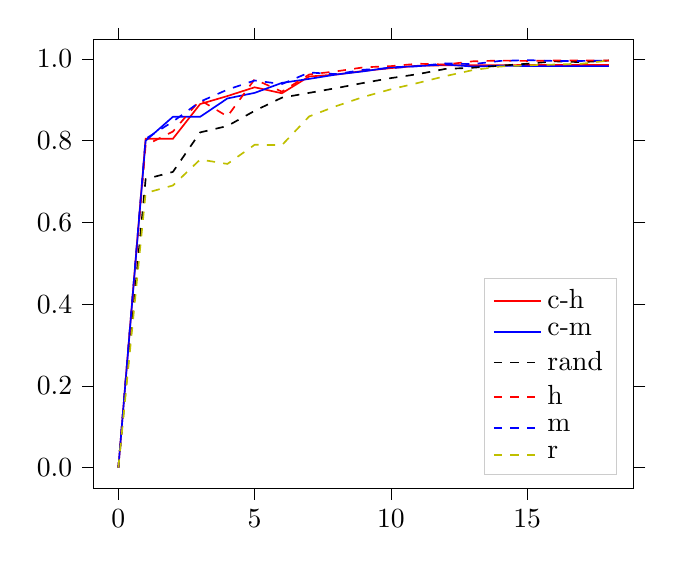
\begin{tikzpicture}

\definecolor{color0}{rgb}{0.75,0.75,0}

\begin{axis}[
legend cell align={left},
legend style={
  fill opacity=0.8,
  draw opacity=1,
  text opacity=1,
  at={(0.97,0.03)},
  anchor=south east,
  draw=white!80!black
},
tick align=outside,
tick pos=both,
x grid style={white!69.0196078431373!black},
xmin=-0.9, xmax=18.9,
xtick style={color=black},
y grid style={white!69.0196078431373!black},
ymin=-0.049853515625, ymax=1.046923828125,
ytick style={color=black},
ytick={-0.2,0,0.2,0.4,0.6,0.8,1,1.2},
yticklabels={−0.2,0.0,0.2,0.4,0.6,0.8,1.0,1.2}
]
\addplot [semithick, red]
table {%
0 0
1 0.8046875
2 0.8046875
3 0.8896484375
4 0.9091796875
5 0.9306640625
6 0.916015625
7 0.95703125
8 0.9619140625
9 0.970703125
10 0.9775390625
11 0.9833984375
12 0.984375
13 0.984375
14 0.984375
15 0.9853515625
16 0.9853515625
17 0.9853515625
18 0.9853515625
};
\addlegendentry{c-h}
\addplot [semithick, blue]
table {%
0 0
1 0.7998046875
2 0.8583984375
3 0.8583984375
4 0.9033203125
5 0.9169921875
6 0.94140625
7 0.951171875
8 0.9619140625
9 0.9697265625
10 0.9794921875
11 0.982421875
12 0.986328125
13 0.9814453125
14 0.9833984375
15 0.982421875
16 0.982421875
17 0.982421875
18 0.982421875
};
\addlegendentry{c-m}
\addplot [semithick, black, dashed]
table {%
0 0
1 0.7060546875
2 0.7236328125
3 0.8203125
4 0.8359375
5 0.873046875
6 0.9052734375
7 0.9169921875
8 0.9287109375
9 0.94140625
10 0.953125
11 0.962890625
12 0.9755859375
13 0.978515625
14 0.9833984375
15 0.98828125
16 0.994140625
17 0.9921875
18 0.99609375
};
\addlegendentry{rand}
\addplot [semithick, red, dashed]
table {%
0 0
1 0.7890625
2 0.822265625
3 0.8994140625
4 0.859375
5 0.9501953125
6 0.919921875
7 0.9619140625
8 0.9697265625
9 0.9794921875
10 0.982421875
11 0.98828125
12 0.986328125
13 0.994140625
14 0.99609375
15 0.9951171875
16 0.99609375
17 0.99609375
18 0.99609375
};
\addlegendentry{h}
\addplot [semithick, blue, dashed]
table {%
0 0
1 0.8046875
2 0.8466796875
3 0.8955078125
4 0.9248046875
5 0.947265625
6 0.9384765625
7 0.966796875
8 0.962890625
9 0.9736328125
10 0.9775390625
11 0.982421875
12 0.9892578125
13 0.9873046875
14 0.9951171875
15 0.9970703125
16 0.9951171875
17 0.9951171875
18 0.99609375
};
\addlegendentry{m}
\addplot [semithick, color0, dashed]
table {%
0 0
1 0.671875
2 0.6904296875
3 0.75390625
4 0.7431640625
5 0.7900390625
6 0.7890625
7 0.859375
8 0.884765625
9 0.9072265625
10 0.92578125
11 0.94140625
12 0.9580078125
13 0.97265625
14 0.9814453125
15 0.984375
16 0.986328125
17 0.98828125
18 0.99609375
};
\addlegendentry{r}
\end{axis}

\end{tikzpicture}

% This file was created by tikzplotlib v0.9.8.
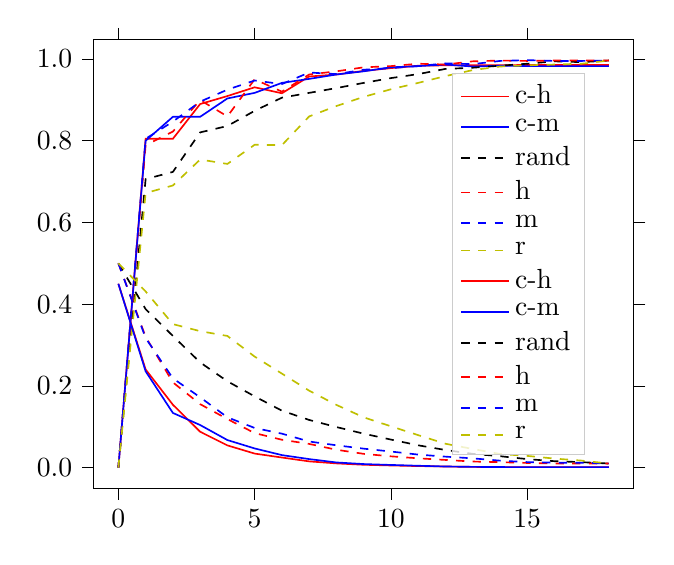
\begin{tikzpicture}

\definecolor{color0}{rgb}{0.75,0.75,0}

\begin{axis}[
legend cell align={left},
legend style={
  fill opacity=0.8,
  draw opacity=1,
  text opacity=1,
  at={(0.91,0.5)},
  anchor=east,
  draw=white!80!black
},
tick align=outside,
tick pos=both,
x grid style={white!69.0196078431373!black},
xmin=-0.9, xmax=18.9,
xtick style={color=black},
y grid style={white!69.0196078431373!black},
ymin=-0.049853515625, ymax=1.046923828125,
ytick style={color=black},
ytick={-0.2,0,0.2,0.4,0.6,0.8,1,1.2},
yticklabels={−0.2,0.0,0.2,0.4,0.6,0.8,1.0,1.2}
]
\addplot [semithick, red]
table {%
0 0
1 0.8046875
2 0.8046875
3 0.8896484375
4 0.9091796875
5 0.9306640625
6 0.916015625
7 0.95703125
8 0.9619140625
9 0.970703125
10 0.9775390625
11 0.9833984375
12 0.984375
13 0.984375
14 0.984375
15 0.9853515625
16 0.9853515625
17 0.9853515625
18 0.9853515625
};
\addlegendentry{c-h}
\addplot [semithick, blue]
table {%
0 0
1 0.7998046875
2 0.8583984375
3 0.8583984375
4 0.9033203125
5 0.9169921875
6 0.94140625
7 0.951171875
8 0.9619140625
9 0.9697265625
10 0.9794921875
11 0.982421875
12 0.986328125
13 0.9814453125
14 0.9833984375
15 0.982421875
16 0.982421875
17 0.982421875
18 0.982421875
};
\addlegendentry{c-m}
\addplot [semithick, black, dashed]
table {%
0 0
1 0.7060546875
2 0.7236328125
3 0.8203125
4 0.8359375
5 0.873046875
6 0.9052734375
7 0.9169921875
8 0.9287109375
9 0.94140625
10 0.953125
11 0.962890625
12 0.9755859375
13 0.978515625
14 0.9833984375
15 0.98828125
16 0.994140625
17 0.9921875
18 0.99609375
};
\addlegendentry{rand}
\addplot [semithick, red, dashed]
table {%
0 0
1 0.7890625
2 0.822265625
3 0.8994140625
4 0.859375
5 0.9501953125
6 0.919921875
7 0.9619140625
8 0.9697265625
9 0.9794921875
10 0.982421875
11 0.98828125
12 0.986328125
13 0.994140625
14 0.99609375
15 0.9951171875
16 0.99609375
17 0.99609375
18 0.99609375
};
\addlegendentry{h}
\addplot [semithick, blue, dashed]
table {%
0 0
1 0.8046875
2 0.8466796875
3 0.8955078125
4 0.9248046875
5 0.947265625
6 0.9384765625
7 0.966796875
8 0.962890625
9 0.9736328125
10 0.9775390625
11 0.982421875
12 0.9892578125
13 0.9873046875
14 0.9951171875
15 0.9970703125
16 0.9951171875
17 0.9951171875
18 0.99609375
};
\addlegendentry{m}
\addplot [semithick, color0, dashed]
table {%
0 0
1 0.671875
2 0.6904296875
3 0.75390625
4 0.7431640625
5 0.7900390625
6 0.7890625
7 0.859375
8 0.884765625
9 0.9072265625
10 0.92578125
11 0.94140625
12 0.9580078125
13 0.97265625
14 0.9814453125
15 0.984375
16 0.986328125
17 0.98828125
18 0.99609375
};
\addlegendentry{r}
\addplot [semithick, red]
table {%
0 0.449999999999992
1 0.240321093750003
2 0.154068750000002
3 0.0879601562499998
4 0.0545979492187504
5 0.0345669921874999
6 0.0248742187499998
7 0.0154591796875
8 0.0104958984375
9 0.00716503906250006
10 0.00544667968750006
11 0.00400634765625
12 0.00290869140625
13 0.00200585937499999
14 0.00137460937499999
15 0.00145478515624999
16 0.00144414062499999
17 0.00143984374999999
18 0.00143974609374999
};
\addlegendentry{c-h}
\addplot [semithick, blue]
table {%
0 0.449999999999992
1 0.235816308593751
2 0.133981542968751
3 0.1044369140625
4 0.0676275390624998
5 0.0471173828125
6 0.0308186523437499
7 0.0210914062499999
8 0.0128307617187499
9 0.00890488281249997
10 0.00674853515625
11 0.00476650390625
12 0.00295224609375002
13 0.00205888671875
14 0.00155673828125
15 0.00136240234375
16 0.00144453125
17 0.0014396484375
18 0.001439453125
};
\addlegendentry{c-m}
\addplot [semithick, black, dashed]
table {%
0 0.5
1 0.38800205078125
2 0.32236396484375
3 0.25762578125
4 0.21144267578125
5 0.1745076171875
6 0.139484375
7 0.116849609375
8 0.09946396484375
9 0.0832636718750001
10 0.0688158203125002
11 0.0547997070312502
12 0.0433041015625001
13 0.0339080078125
14 0.0281607421874999
15 0.0210115234374999
16 0.0159416015625
17 0.013575390625
18 0.0101943359375
};
\addlegendentry{rand}
\addplot [semithick, red, dashed]
table {%
0 0.5
1 0.3201904296875
2 0.20880224609375
3 0.155491015625001
4 0.118972656250001
5 0.0846564453125002
6 0.0683878906250001
7 0.0581800781250001
8 0.04395986328125
9 0.0338941406249999
10 0.0278213867187499
11 0.0230004882812499
12 0.01899560546875
13 0.0150919921875
14 0.0135923828125
15 0.0116212890625
16 0.01030810546875
17 0.0101529296875
18 0.0101943359375
};
\addlegendentry{h}
\addplot [semithick, blue, dashed]
table {%
0 0.5
1 0.317187499999997
2 0.218678808593748
3 0.172235253906248
4 0.123334277343749
5 0.0972216796875
6 0.0832712890624999
7 0.0641038085937499
8 0.0548044921874999
9 0.04663076171875
10 0.03955947265625
11 0.0320949218749999
12 0.0270456054687499
13 0.0228884765625
14 0.0172658203125
15 0.01367705078125
16 0.0123193359375
17 0.01206787109375
18 0.0101943359375
};
\addlegendentry{m}
\addplot [semithick, color0, dashed]
table {%
0 0.5
1 0.431250000000002
2 0.351269531249998
3 0.3340296875
4 0.322312109375
5 0.27181015625
6 0.23018603515625
7 0.188451464843749
8 0.15362529296875
9 0.123285546875
10 0.10120791015625
11 0.0796852539062503
12 0.0586057617187502
13 0.0458888671875001
14 0.0336228515625
15 0.02890341796875
16 0.022294140625
17 0.01733564453125
18 0.0101943359375
};
\addlegendentry{r}
\end{axis}

\end{tikzpicture}

\caption{Aggregated Accuracy (left) and Brier score (right) for a multi-skill TA}
\label{fig:multi}
\end{figure}

\section{Outlooks and Conclusions}\label{sec:conc}
A new score for adaptive testing in Bayesian and credal networks has been proposed.
\bibliographystyle{splncs04}
\bibliography{biblio}
\end{document}